\documentclass[tikz]{standalone}
\usetikzlibrary{decorations.pathreplacing,calligraphy,calc,graphs, shapes, backgrounds}
\graphicspath{{../images/}}
\usepackage[russian]{babel} % поддержка кириллицы
\usepackage[utf8]{inputenc} % кодировка UTF-8
\usepackage[X2,T2A]{fontenc}
\usepackage{fontspec}
\usepackage{amsmath, amssymb}
\setmainfont{Open Sans}


\begin{document}
\begin{tikzpicture}
    % Include the image in a node
    \node [above right, inner sep=0] (image) at (0,0)
    {\centering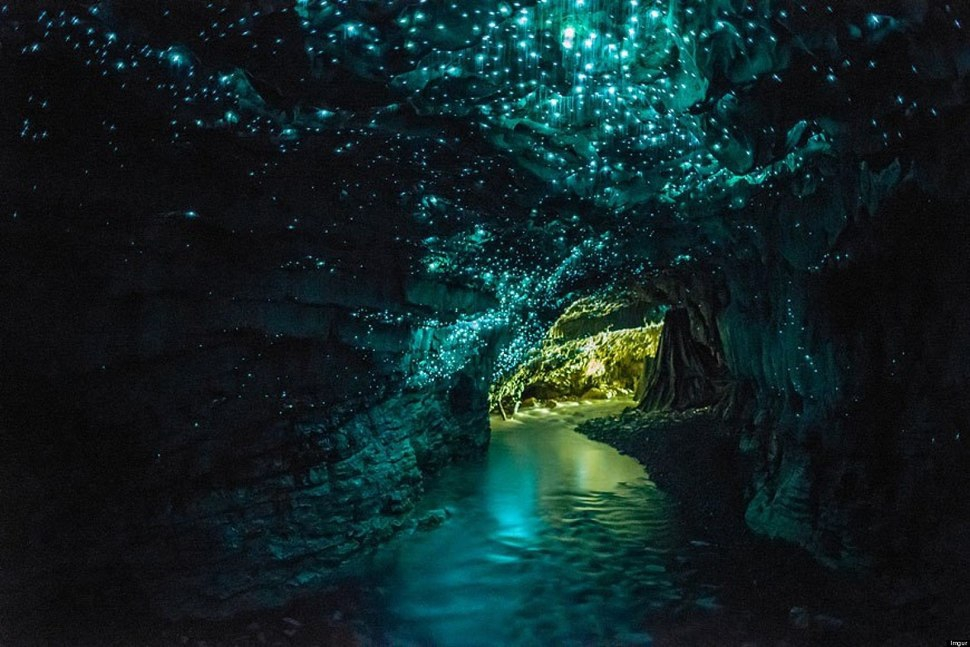
\includegraphics[height=4cm,width=1\textwidth,keepaspectratio]{surface_types/splash.png}};
    % Create scope with normalized axes
    \begin{scope}[
            x={($ 0.1*(image.south east)$)},
            y={($ 0.1*(image.north west)$)}]
        % Labels
        \draw[stealth-, very thick,green] (5,2) -- ++(-2,+1)
        node[rounded corners=3pt,left,black,fill=white]{\tiny Лужа};
    \end{scope}
\end{tikzpicture}

\begin{tikzpicture}
    % Include the image in a node
    \node [above right, inner sep=0] (image) at (0,0)
    {\centering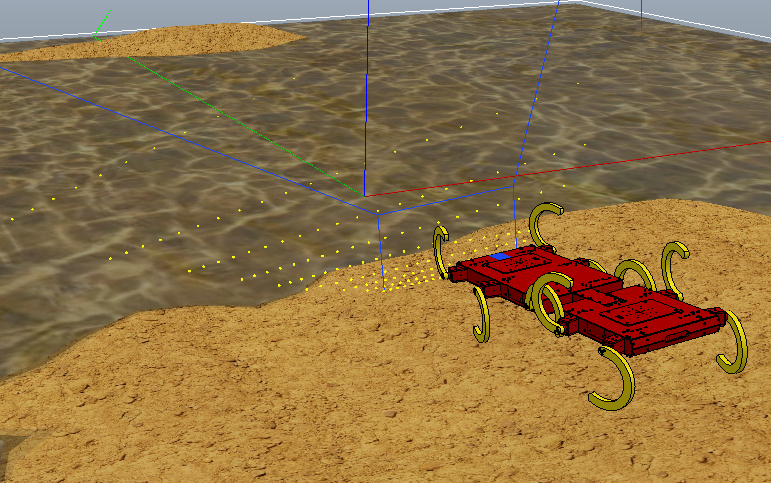
\includegraphics[height=3.5cm,width=1\textwidth,keepaspectratio]{terrain_w_water1.png}};
    % Create scope with normalized axes
    \begin{scope}[
            x={($ 0.1*(image.south east)$)},
            y={($ 0.1*(image.north west)$)}]
        \draw[stealth-, very thick,green] (6,8) -- ++(2,1)
        node[rounded corners=3pt,right,black,fill=white]{\tiny Вода};

        \draw[stealth-, very thick,green] (0.5,5.5) -- (3,2);
        \draw[stealth-, very thick,green] (2.5,4.2) -- (3,2);
        \draw[stealth-, very thick,green] (4.5,4) -- (3,2)
        node[rounded corners=3pt,below,black,fill=white]{\tiny Лазер Лидара};
    \end{scope}
\end{tikzpicture}

\begin{tikzpicture}
    % Include the image in a node
    \node [above right, inner sep=0] (image) at (0,0)
    {\centering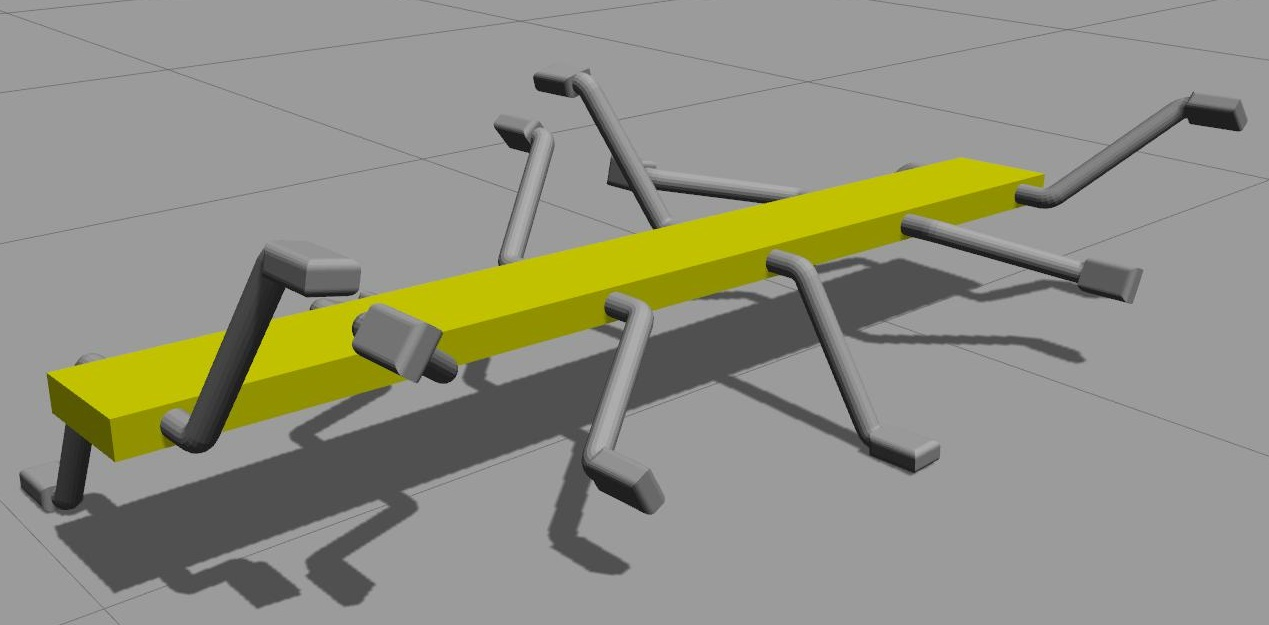
\includegraphics[height=3cm,width=1\textwidth,keepaspectratio]{best_gen_robot.jpg}};
    % Create scope with normalized axes
    \begin{scope}[
            x={($ 0.1*(image.south east)$)},
            y={($ 0.1*(image.north west)$)}]
        % Labels
        \draw [green, very thick,
            decorate,
            decoration = {brace,
                    raise=5pt,
                    amplitude=5pt,
                    aspect=0.5}] (1.4,3.6) --  (8.1,6.8)
        node[rounded corners=3pt, pos=0.5,above left =14pt,black,fill=white]{\tiny $(\gamma - 1) h_{\text{leg}}sin(\alpha)$};

        \draw[stealth-, very thick,green] (9.5,7.8) -- (7.8,1.94);
        \draw[stealth-, very thick,green] (1.5,2.8) -- (7,1)
        node[rounded corners=3pt,right,black,fill=white]{\tiny $\gamma = 6$};

        \draw[thin,green] (6.7,4) -- (5.75,9);
        \draw[thin,green] (4.85,3.5) -- (5.75,9);
        \draw[thin,green,stealth-stealth] (6.32,6) arc (-79.2:-99.2:3) node [rounded corners=3pt,below = 2pt,black,fill=white, midway] {\tiny $\alpha$};
    \end{scope}
\end{tikzpicture}

\begin{tikzpicture}
    % Include the image in a node
    \node [above right, inner sep=0] (image) at (0,0)
    {\centering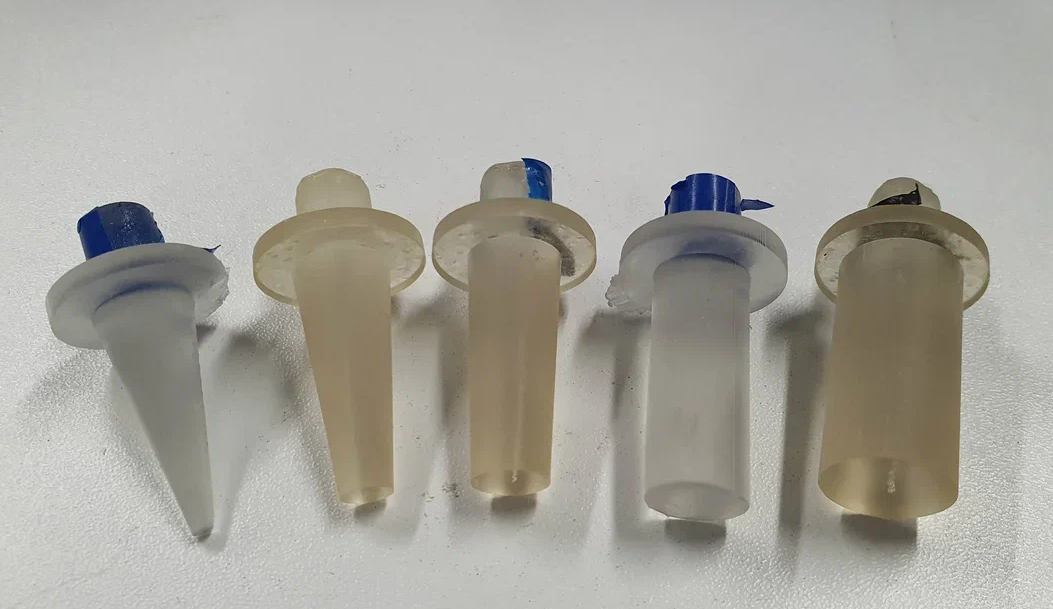
\includegraphics[height=3cm,width=1\textwidth,keepaspectratio]{all_end_effectors.png}};
    % Create scope with normalized axes
    \begin{scope}[
            x={($ 0.1*(image.south east)$)},
            y={($ 0.1*(image.north west)$)}]
        % Labels
        \node[rounded corners=3pt,black,fill=white] at (1.1,7.4){\tiny 2 мм };
        \node[rounded corners=3pt,black,fill=white] at (3.1,7.9){\tiny 6 мм };
        \node[rounded corners=3pt,black,fill=white] at (4.9,8.1){\tiny 8 мм };
        \node[rounded corners=3pt,black,fill=white] at (6.7,7.9){\tiny 12 мм };
        \node[rounded corners=3pt,black,fill=white] at (8.6,7.9){\tiny 15 мм };
    \end{scope}
\end{tikzpicture}

\begin{tikzpicture}
    % Include the image in a node
    \node [
        above right,
        inner sep=0] (image) at (0,0) {\centering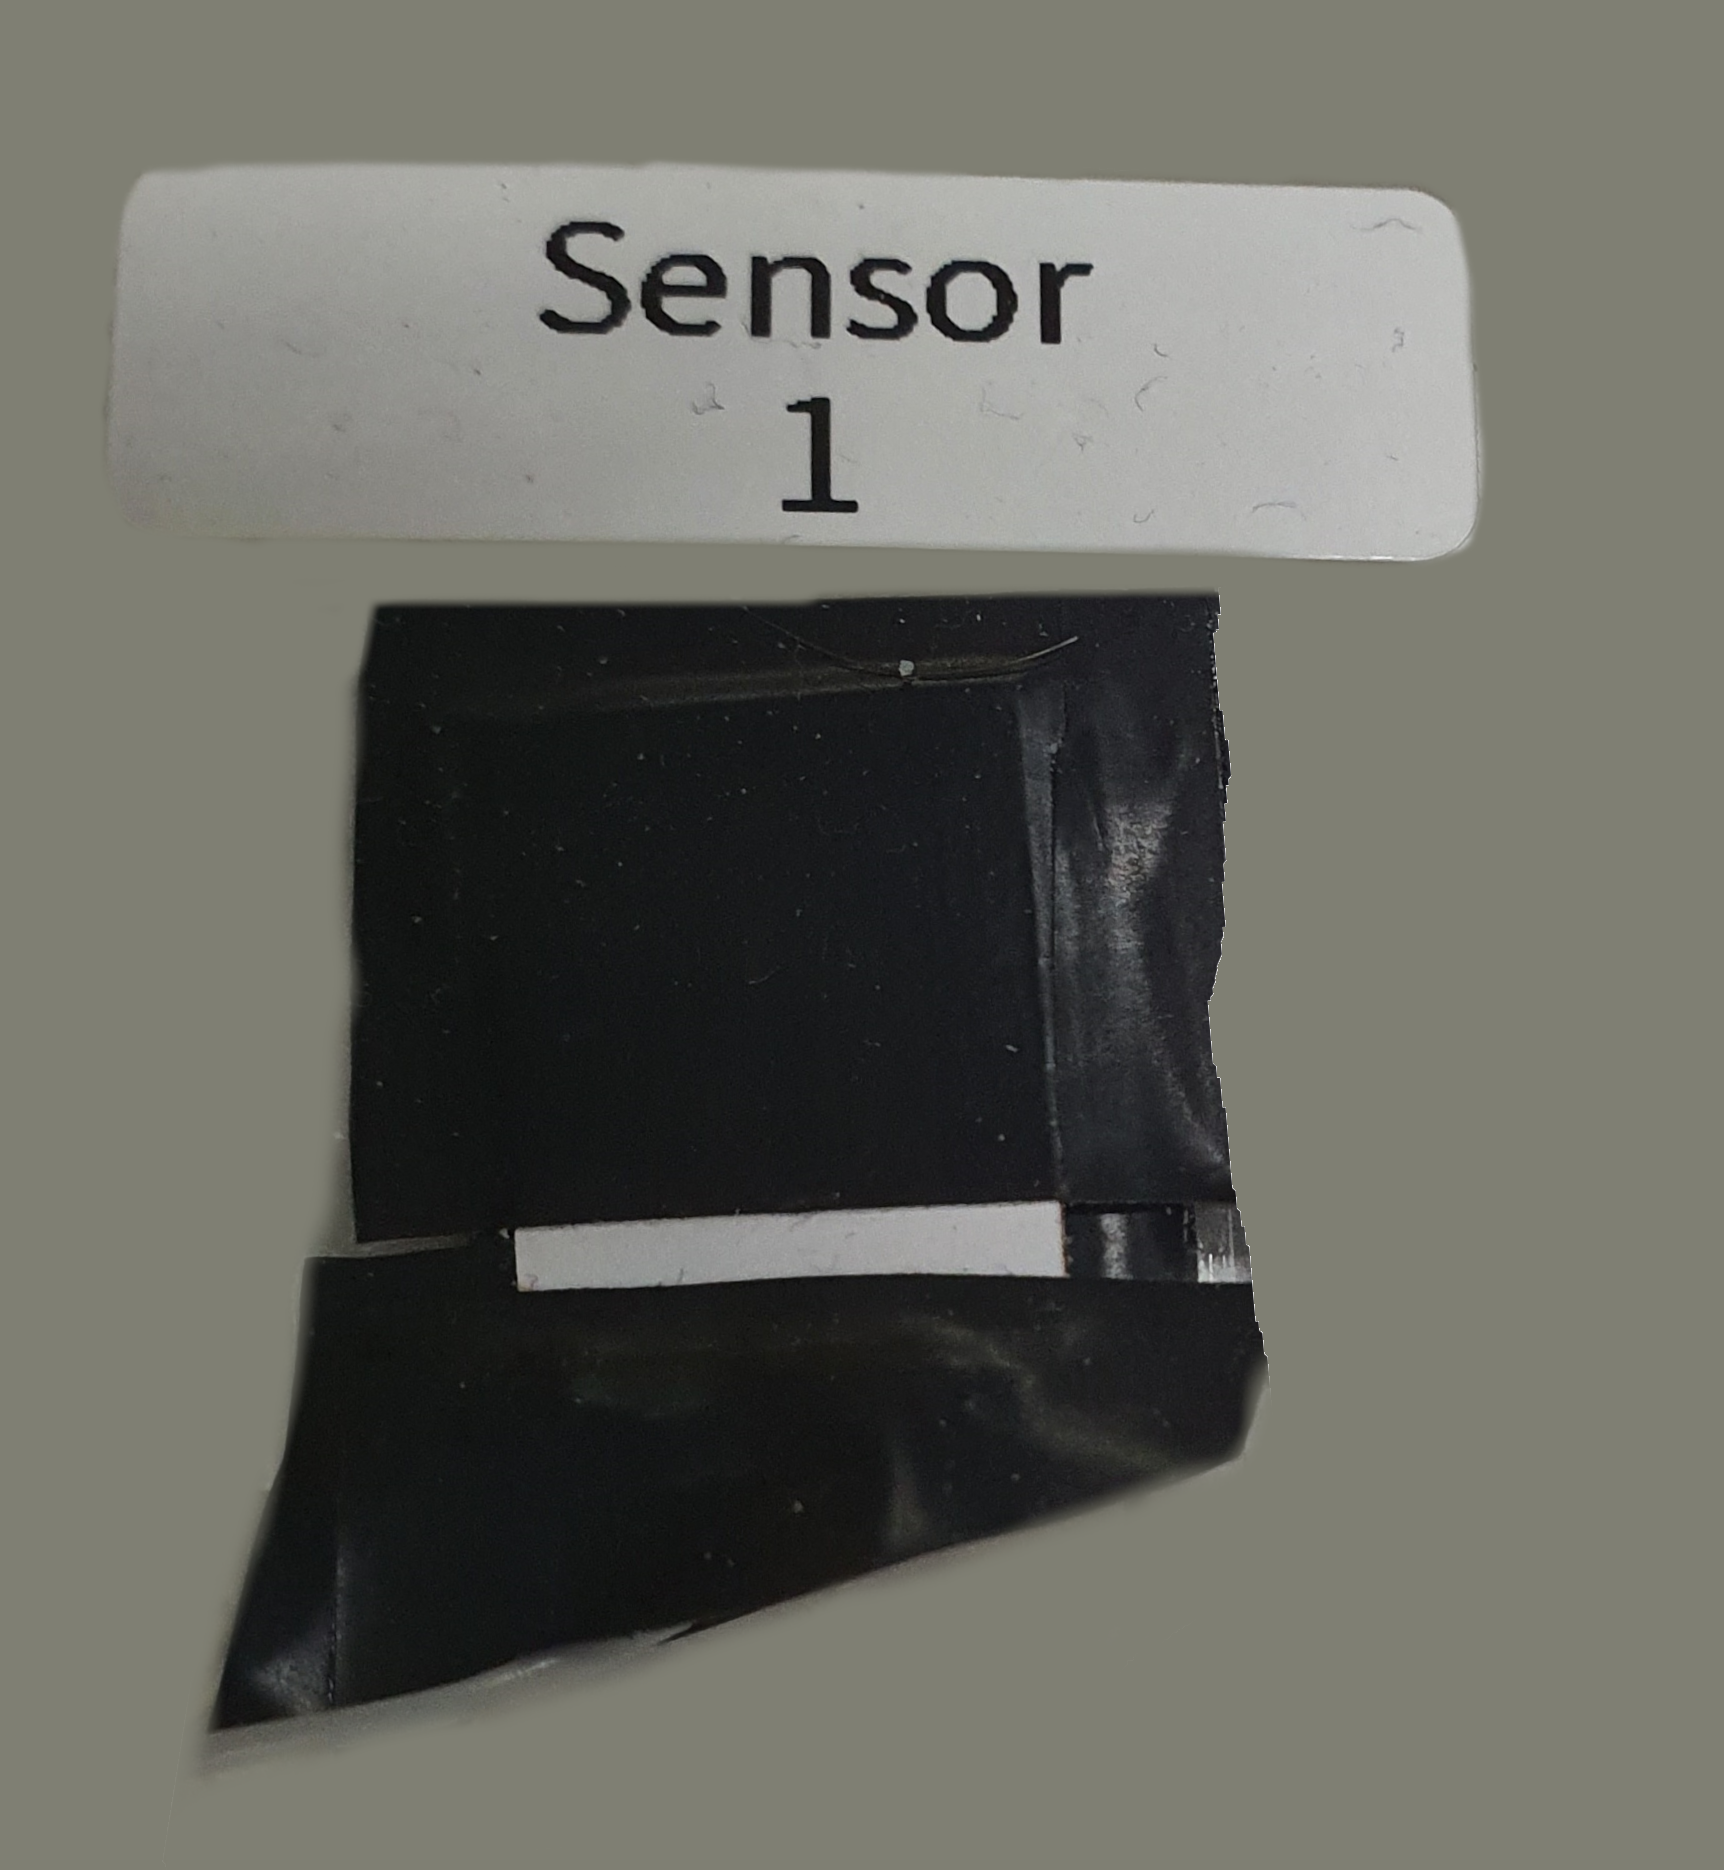
\includegraphics[height=5cm,width=1\textwidth,keepaspectratio]{sensors_grid.png}};

    % Create scope with normalized axes
    \begin{scope}[
            x={($0.1*(image.south east)$)},
            y={($0.1*(image.north west)$)}]
        % Labels
        % Simple brace
        \draw [green, very thick,
            decorate,
            decoration = {brace,
                    raise=5pt,
                    amplitude=5pt,
                    aspect=0.5}] (6,3.7) --  (3,3.7)
        node[pos=0.5,below=10pt,green]{$15\ \text{мм}$};

        \draw [green, very thick,
            decorate,
            decoration = {brace, mirror,
                    raise=5pt,
                    amplitude=5pt,
                    aspect=0.5}] (6,3.6) --  (6,6.4)
        node[pos=0.5,right=10pt,green]{$15\ \text{мм}$};

        \draw[green,step=1,xshift=34, yshift=43]  (0.5,0.5) grid +(3,3);

        \node[circle,fill=green,scale=0.4] at (3.3,6.27){\small 1};
        \node[circle,fill=green,scale=0.4] at (5.92,3.7){\small 16};
    \end{scope}
\end{tikzpicture}


\begin{tikzpicture}
    % Include the image in a node
    \node [above right, inner sep=0] (image) at (0,0)
    {\centering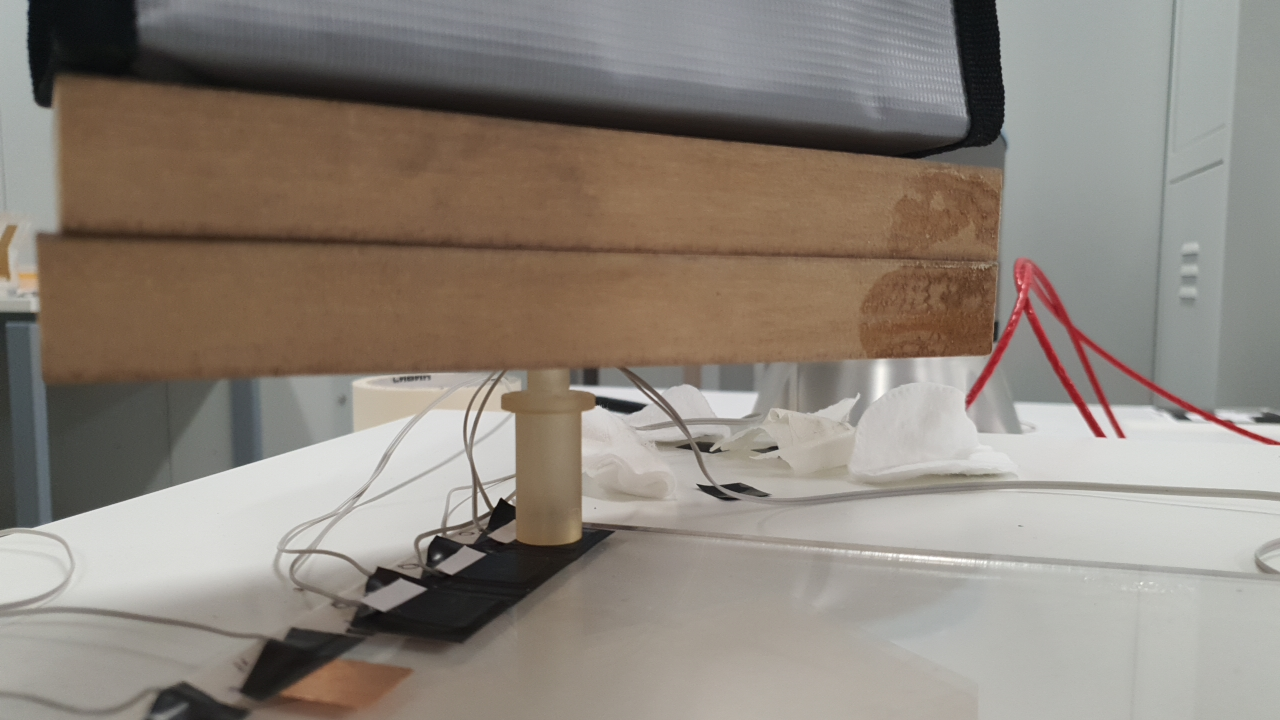
\includegraphics[height=3.4cm,width=1\textwidth,keepaspectratio]{static_load_meh.JPG}};
    % Create scope with normalized axes
    \begin{scope}[
            x={($ 0.1*(image.south east)$)},
            y={($ 0.1*(image.north west)$)}]
        \draw[latex-, very thick,green] (4.3,2.3) -- (5,1.6)
        node[rounded corners=3pt,below right,black,fill=white]{\tiny Исследуемый датчик};

        \draw[latex-, very thick,green] (4.3,3.5) -- (5.5,2.45)
        node[rounded corners=3pt,right,black,fill=white]{\tiny \O \ 15 мм насадка};

        \draw[latex-, very thick,green] (6,6) -- (6.4,4.9)
        node[rounded corners=3pt,below right,black,fill=white]{\tiny Известная нагрузка};
    \end{scope}
\end{tikzpicture}




\begin{tikzpicture}

    % Include the image in a node
    \node [
        above right,
        inner sep=0] (image) at (0,0) {\centering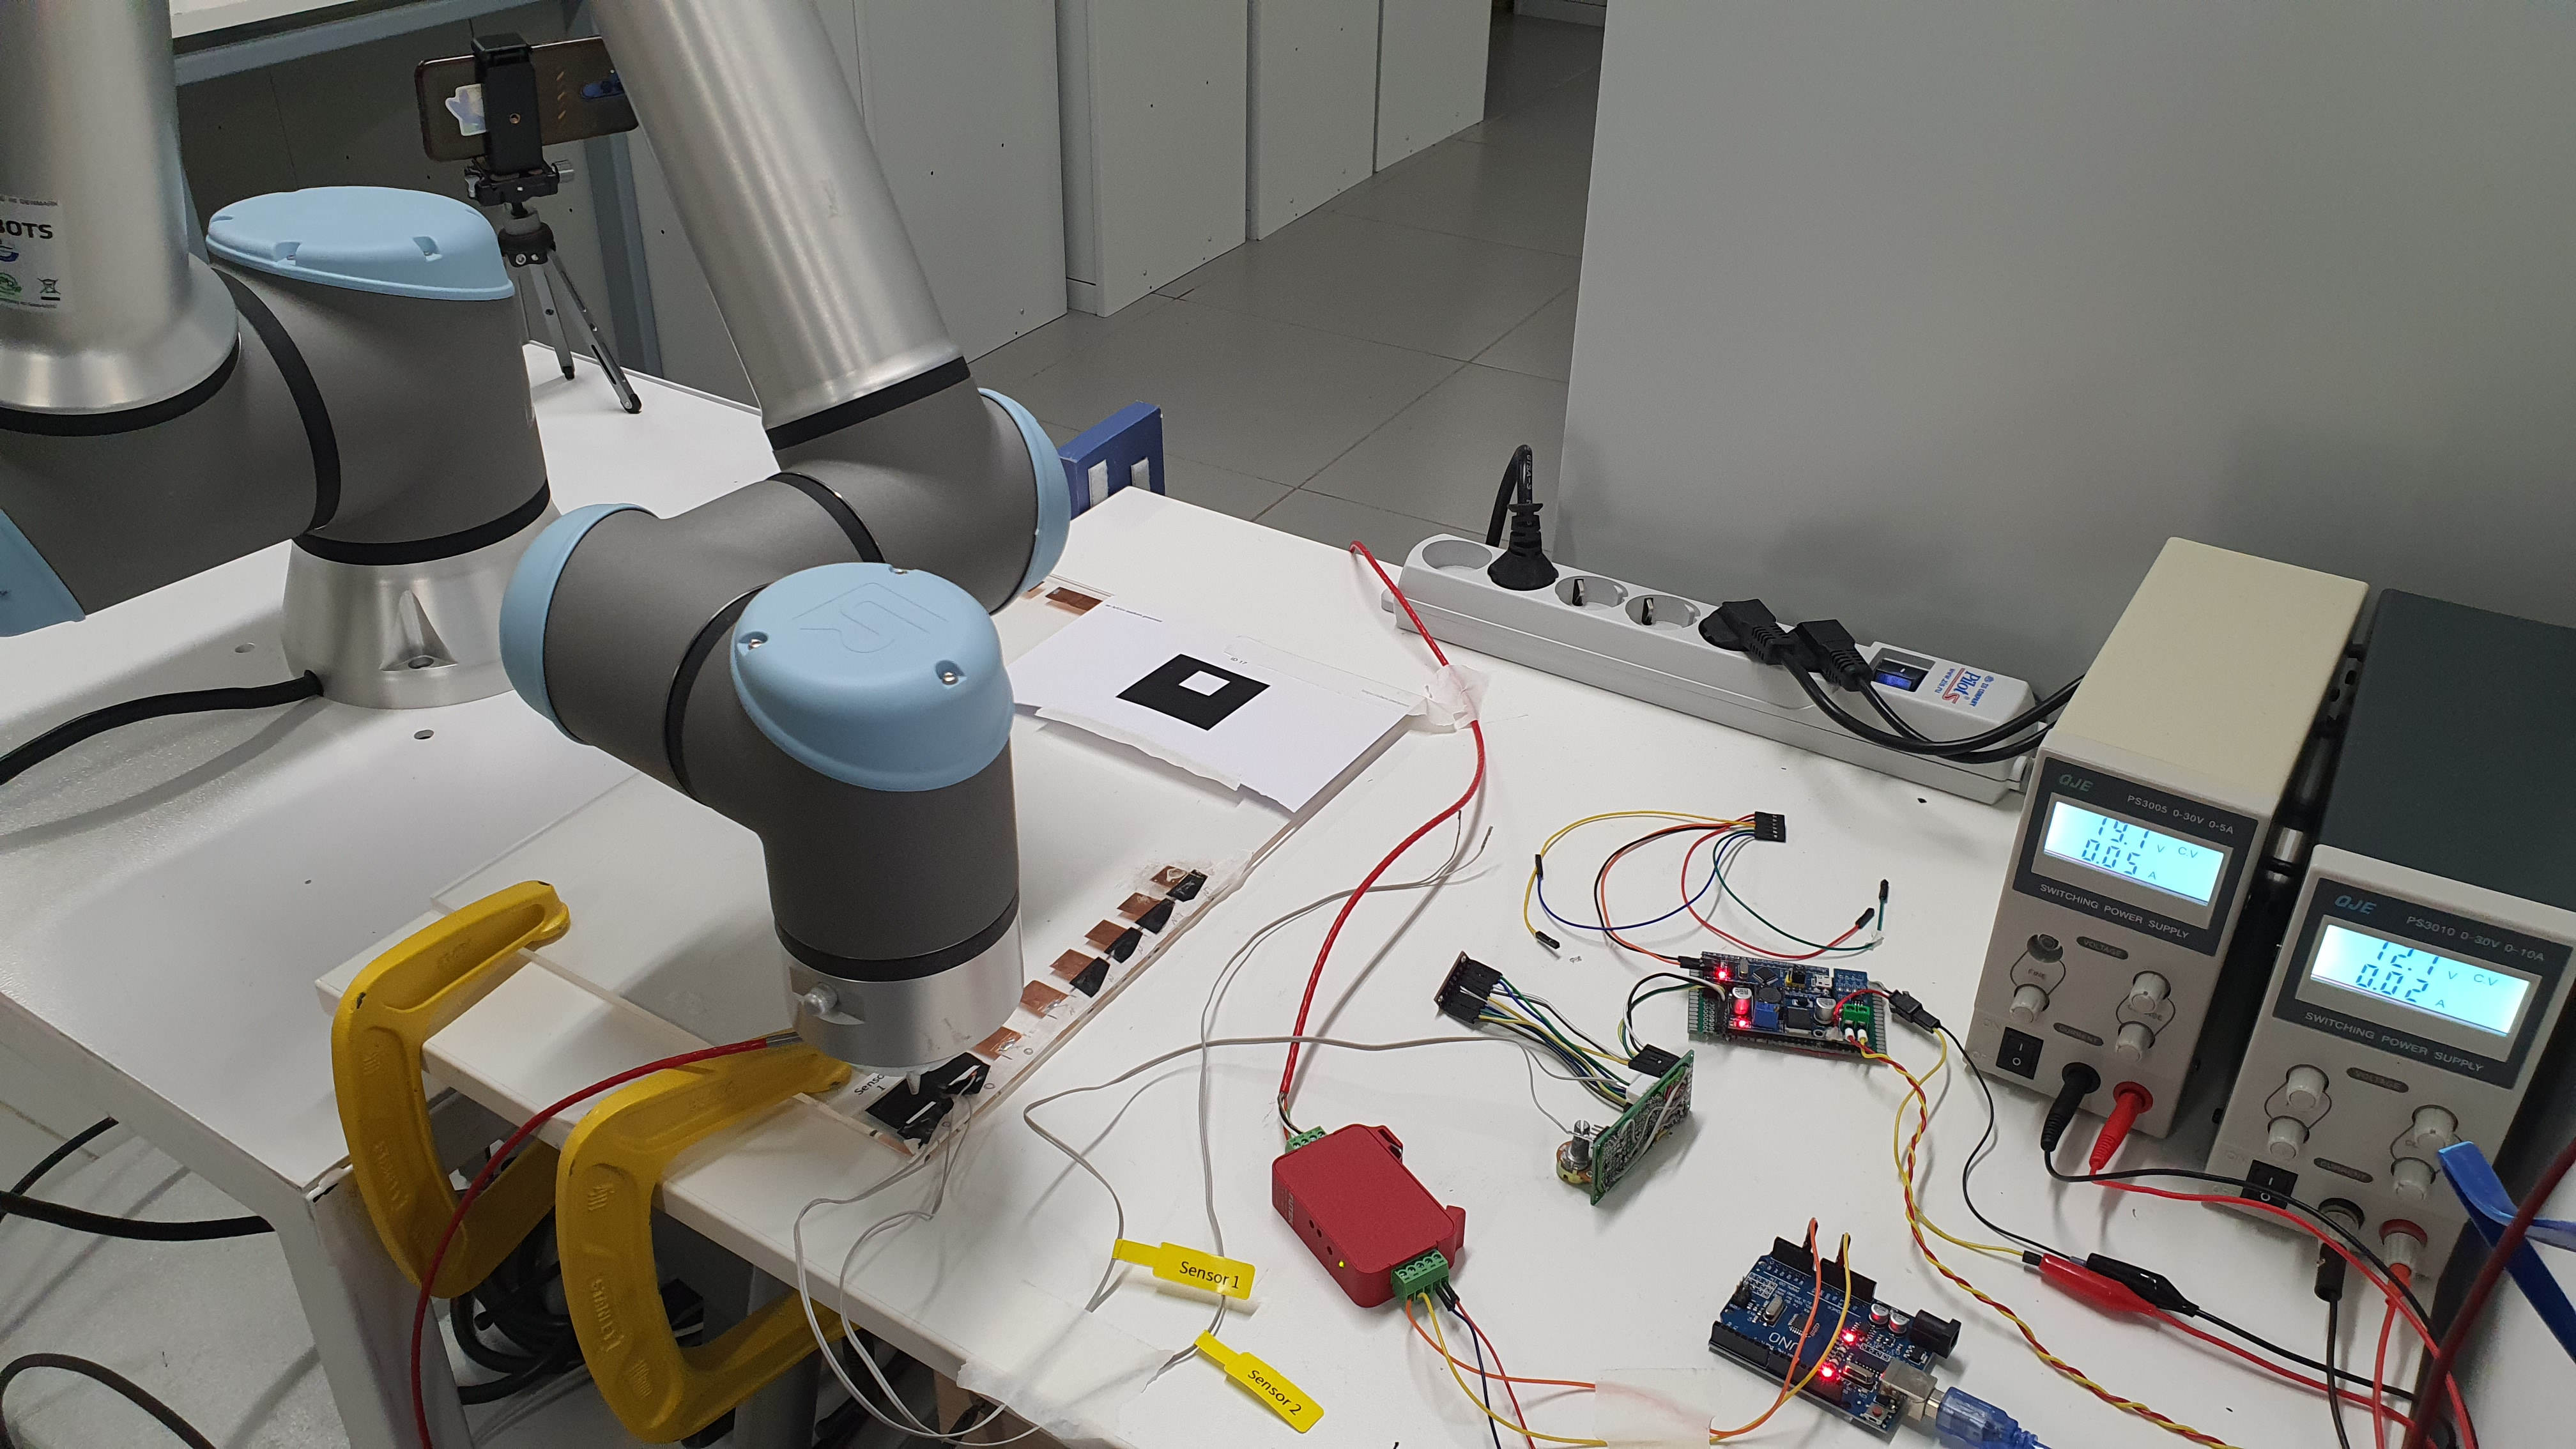
\includegraphics[height=6cm,width=1\textwidth,keepaspectratio]{exp_stand1}};

    % Create scope with normalized axes
    \begin{scope}[
            x={($0.1*(image.south east)$)},
            y={($0.1*(image.north west)$)}]
        \draw[latex-, very thick,green] (3.5,2.2) -- (3.5,1)
        node[rounded corners=3pt,below left,black,fill=white]{\small Исследуемые датчики};

        \draw[stealth-, very thick,green] (3.5,2.6) -- ++(-0.7,+0.5)
        node[rounded corners=3pt,left,black,fill=white]{\small Датчик силы};

        \draw[stealth-, very thick,green] (6.5,3) -- (7,6)
        node[rounded corners=3pt,above right,black,fill=white]{\small Печатная плата};

        \draw[stealth-, very thick,green] (7.2,1.5) -- (8,5)
        node[rounded corners=3pt,above right,black,fill=white]{\small Контроллер};

        \draw[stealth-, very thick,green] (2.5,9.5) -- (4,9.5)
        node[rounded corners=3pt,right,black,fill=white]{\small Камера};

        \draw[very thick,green] (0.5,2.5) rectangle (4.2,9)
        node[below left,black,fill=green]{\small UR10e};

        \draw[latex-, very thick,green] (4.5,7.2) edge (5.5,7.5)
        (4.8,5.3) -- (5.5,7.5)
        node[rounded corners=3pt,above,black,fill=white]{\small Маркеры Aruco};
    \end{scope}

\end{tikzpicture}

\begin{tikzpicture}
    % Include the image in a node
    \node [above right, inner sep=0] (image) at (0,0)
    {\centering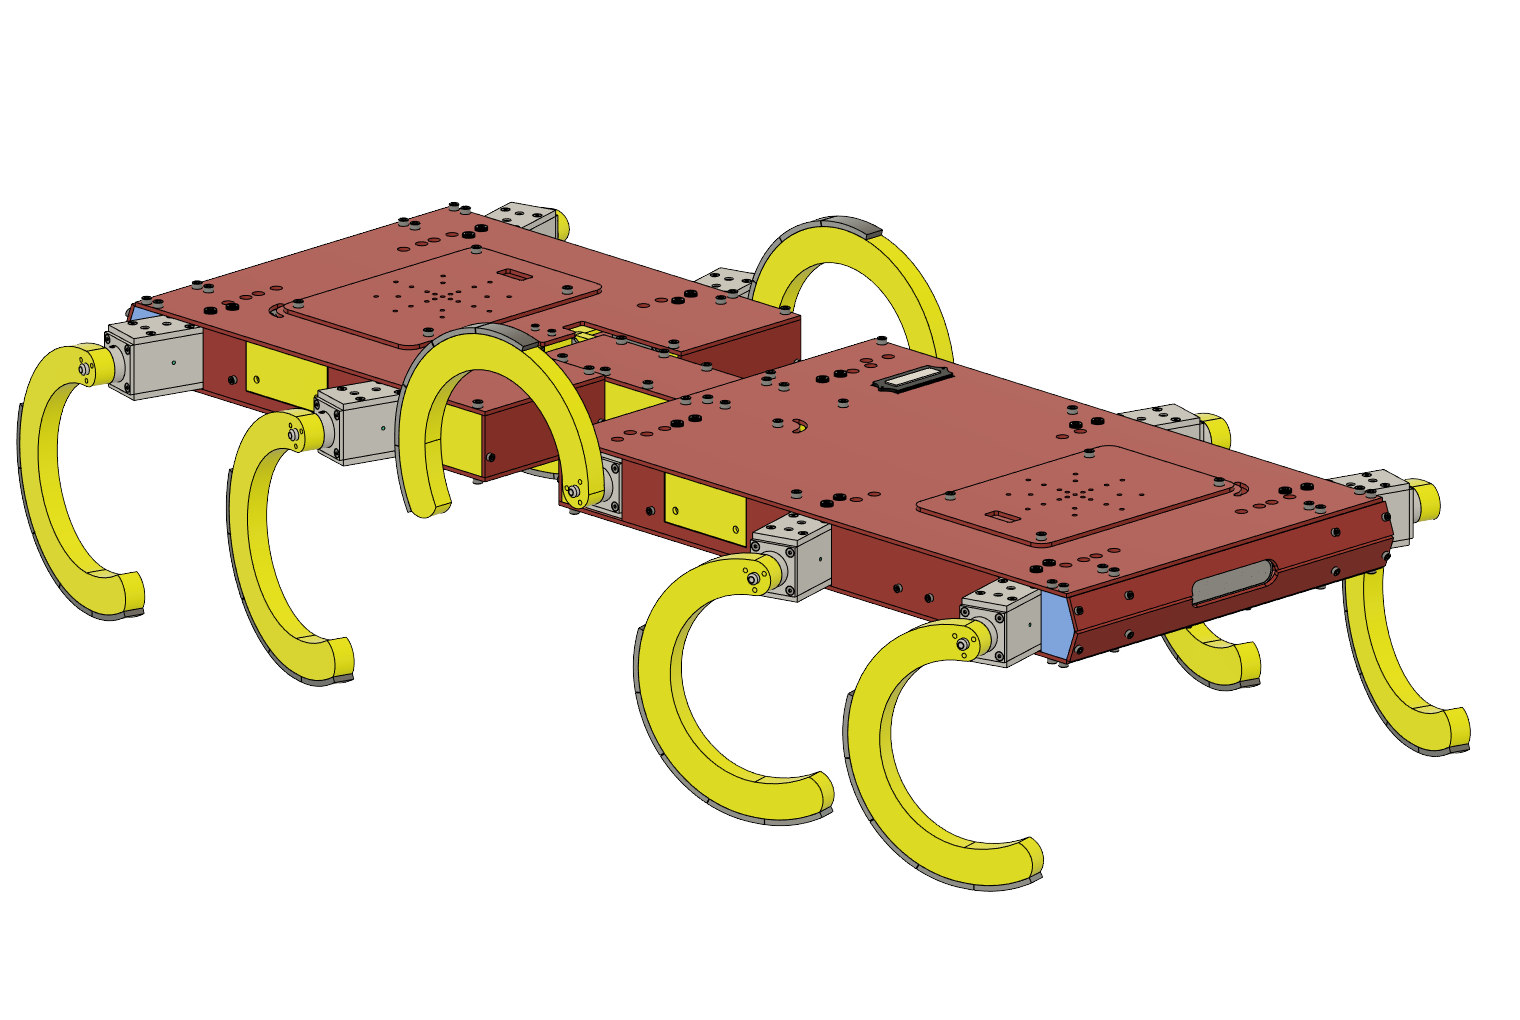
\includegraphics[height=4.5cm,width=1\textwidth,keepaspectratio]{StriRus_10_legs_15_angle_v4.png}};
    % Create scope with normalized axes
    \begin{scope}[
            x={($ 0.1*(image.south east)$)},
            y={($ 0.1*(image.north west)$)}]
        % Grid and axes' labels
        % \draw[lightgray,step=1] (image.south west) grid (image.north east);
        % \foreach \x in {0,1,...,10} { \node [below] at (\x,0) {\x}; }
        % \foreach \y in {0,1,...,10} { \node [left] at (0,\y) {\y};}

        % Labels

        \coordinate (Xc) at (0.4415/2,-0.2347/2);
        \coordinate (Yc) at (-0.4512/2,-0.2156/2);
        \coordinate (Zc) at (0,0.5/2);
        % Labels
        \tikzstyle{origin} = [rounded corners=2pt, black, fill=gray!40, fill opacity=0.75, text opacity=1, scale=0.8,inner sep=1pt]
        \tikzstyle{transform_text} = [rounded corners=2pt, black, fill=white!85!gray, fill opacity=0.75, text opacity=1, scale=0.8,inner sep=1pt]
        \tikzstyle{transform_arrow} = [thick, green]

        % \coordinate (o_g) at (1,9);
        \node[circle,fill=green,scale=0.25] (o_g) at (1,9){};
        \draw[-stealth, very thick,blue] (o_g) -- ++(Xc);
        \draw[-stealth, very thick,green!70!black] (o_g) -- ++(Yc);
        \draw[-stealth, very thick,red] (o_g) -- ++(Zc);
        \node[origin,above right=3pt] at (o_g){\tiny $\mathbf{O_{glob}}$};

        % \coordinate (o_b) at (2.9,7.05);
        \node[circle,fill=green,scale=0.25] (o_b) at (2.9,7.05){};
        \draw[-stealth, very thick,blue] (o_b) -- ++(Xc);
        \draw[-stealth, very thick,green!70!black] (o_b) -- ++(Yc);
        \draw[-stealth, very thick,red] (o_b) -- ++(Zc);
        \node[origin,above right=2pt] at (o_b){\tiny $\mathbf{O_{base}}$};

        % \coordinate (o_1) at (2.9,6.6);
        \node[circle,fill=green,scale=0.25] (o_1) at (2.9,6.6){};
        \draw[-stealth, very thick,blue] (o_1) -- ++(Xc);
        \draw[-stealth, very thick,green!70!black] (o_1) -- ++(Yc);
        \draw[-stealth, very thick,red] (o_1) -- ++(Zc);
        \node[origin,above right=2pt] at (o_1){\tiny $\mathbf{O_{1}}$};

        % \coordinate (o_2) at (4,6);
        \node[circle,fill=green,scale=0.25] (o_2) at (4,6){};
        \draw[-stealth, very thick,blue] (o_2) -- ++(Xc);
        \draw[-stealth, very thick,green!70!black] (o_2) -- ++(Yc)
        node[origin,below=2pt]{\tiny $\mathbf{\alpha_3}$};
        \draw[-stealth, very thick,red] (o_2) -- ++(Zc);
        \node[origin,above right=2pt] at (o_2){\tiny $\mathbf{O_{2}=O_{3}}$};

        % \coordinate (o_4) at (7.0,4.55);
        \node[circle,fill=green,scale=0.25] (o_4) at (7.0,4.55){};
        \draw[-stealth, very thick,blue] (o_4) -- ++(Xc);
        \draw[-stealth, very thick,green!70!black] (o_4) -- ++(Yc);
        \draw[-stealth, very thick,red] (o_4) -- ++(Zc);
        \node[origin,above right=2pt] at (o_4){\tiny $\mathbf{O_{4}}$};

        % \coordinate (o_5) at (6.7,4.45);
        \node[circle,fill=green,scale=0.25] (o_5) at (6.7,4.45){};
        \draw[-stealth, very thick,blue] (o_5) -- ++(Xc);
        \draw[-stealth, very thick,green!70!black] (o_5) -- ++(Yc);
        \draw[-stealth, very thick,red] (o_5) -- ++(Zc);
        \node[origin,above left=3pt] at (o_5){\tiny $\mathbf{O_{5}=O_{6}}$};

        \coordinate (Xcr) at (0.49/2,0.07/2);
        % \coordinate (Ycr) at (-0.38/2,-0.32/2);
        \coordinate (Ycr) at (-0.24/2,-0.43/2);

        \draw[-stealth, very thick,blue] (o_5) -- ++(Xcr);
        \draw[-stealth, very thick,green!70!black] (o_5) -- ++(Ycr);


        % \coordinate (o_7) at (6.36,3.68);
        \node[circle,fill=green,scale=0.25] (o_7) at (6.36,3.68){};
        \draw[-stealth, very thick, blue] (o_7) -- ++(Xcr);
        \draw[-stealth, very thick, green!70!black] (o_7) -- ++(Ycr)
        node[origin,above left=2pt]{\tiny $\mathbf{\alpha_8}$};
        \draw[-stealth, very thick, red] (o_7) -- ++(Zc);
        \node[origin,below right=3pt] at (o_7){\tiny $\mathbf{O_{7}=O_{8}}$};

        \node[circle, draw ,fill=green,scale=0.4] (s_1) at (6.6,1.3){1};
        \node[circle,draw, fill=green,scale=0.4] (s_3) at (5.85,1.7){3};
        \node[circle,draw, fill=green,scale=0.4] (s_5) at (5.55,2.9){5};

        \draw[-stealth, transform_arrow] (o_g) -- (o_b)
        node[midway,below left=2pt, transform_text]{\tiny $\mathbf{H_{base}^{glob}}$};

        \draw[-stealth, transform_arrow] (o_b) -- (o_1)
        node[midway,left=3pt, transform_text]{\tiny $\mathbf{H_{1}^{base}}$};

        \draw[-stealth, transform_arrow] (o_1) -- (o_2)
        node[midway,below=2pt, transform_text]{\tiny $\mathbf{H_{2}^{1}}$};

        \draw[-stealth, transform_arrow] (o_2) -- (o_4)
        node[midway,below=2pt, transform_text]{\tiny $\mathbf{H_{4}^{3}}$};

        \draw[-stealth, transform_arrow] (o_4) -- (o_5)
        node[midway,below right=2pt, transform_text]{\tiny $\mathbf{H_{5}^{4}}$};

        \draw[-stealth, transform_arrow] (o_5) -- (o_7)
        node[midway,left=3pt, transform_text]{\tiny $\mathbf{H_{7}^{6}}$};

        \draw[-stealth, transform_arrow] (o_7) -- (s_1);
        \draw[-stealth, transform_arrow] (o_7) -- (s_3);
        \draw[-stealth, transform_arrow] (o_7) -- (s_5);
    \end{scope}
\end{tikzpicture}

\begin{tikzpicture}
    % Include the image in a node
    \node [above right, inner sep=0] (image) at (0,0)
    {\centering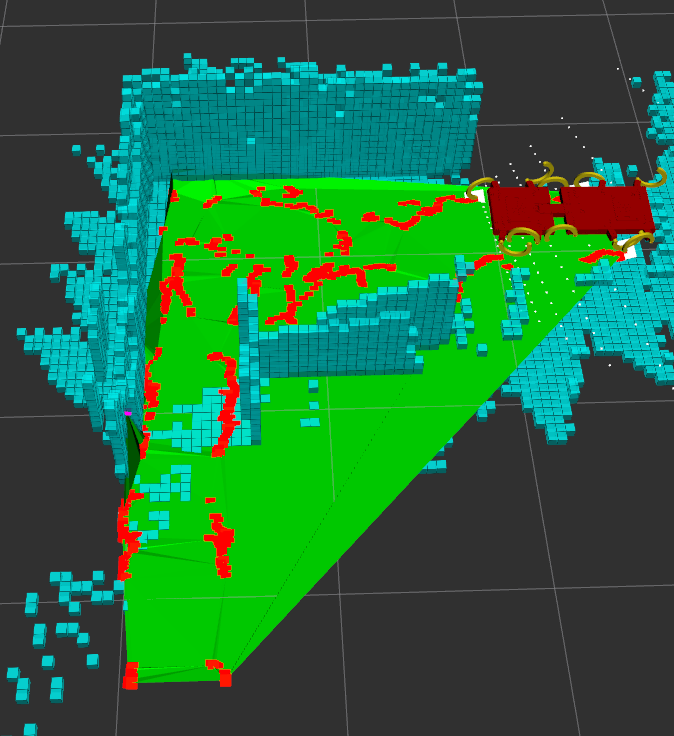
\includegraphics[height=6cm,width=1\textwidth,keepaspectratio]{conv_convex.png}};
    % Create scope with normalized axes
    \begin{scope}[
            x={($ 0.1*(image.south east)$)},
            y={($ 0.1*(image.north west)$)}]
        % Grid and axes' labels
        % \draw[lightgray,step=1] (image.south west) grid (image.north east);
        % \foreach \x in {0,1,...,10} { \node [below] at (\x,0) {\x}; }
        % \foreach \y in {0,1,...,10} { \node [left] at (0,\y) {\y};}

        % Labels
        \draw[stealth-, very thick,green] (5.2,3.5) -- ++(0,-1)
        node[rounded corners=3pt,right,black,fill=white]{\tiny Полученная сетка};

        \draw[stealth-, very thick,green] (5.5,5.5) -- (6.4,4)
        node[rounded corners=3pt,right,black,fill=white]{\tiny Данные лидара};


        \draw[stealth-, very thick,green] (3.4,0.8) -- (5,1);
        \draw[stealth-, very thick,green] (3.4,2.6) -- (5,1)
        node[rounded corners=3pt,right,black,fill=white]{\tiny Следовая дорожка};
    \end{scope}
\end{tikzpicture}

\begin{tikzpicture}
    % Include the image in a node
    \node [above right, inner sep=0] (image) at (0,0)
    {\centering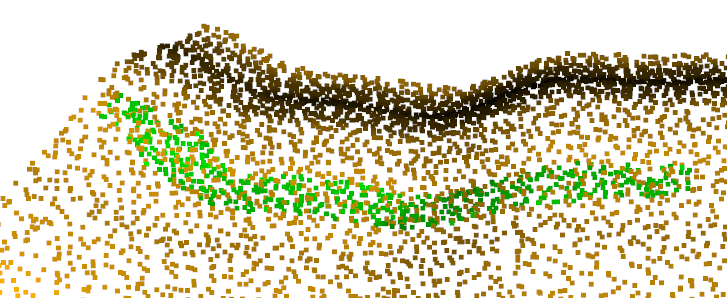
\includegraphics[height=2.8cm,width=1\textwidth,keepaspectratio]{sampled_pcd.png}};
    % Create scope with normalized axes
    \begin{scope}[
            x={($ 0.1*(image.south east)$)},
            y={($ 0.1*(image.north west)$)}]
        % Grid and axes' labels
        % \draw[lightgray,step=1] (image.south west) grid (image.north east);
        % \foreach \x in {0,1,...,10} { \node [below] at (\x,0) {\x}; }
        % \foreach \y in {0,1,...,10} { \node [left] at (0,\y) {\y};}

        % Labels
        \draw[stealth-, very thick,green] (3,8) -- (2,8.5);
        \draw[stealth-, very thick,green] (1,5.5) -- (2,8.5)
        node[rounded corners=3pt,above,black,fill=white]{\tiny Эталонное Облако};

        \draw[stealth-, very thick,green] (5.5,3) -- (5.5,8.5)
        node[rounded corners=3pt,above,black,fill=white]{\tiny Сгенерированное Облако};
    \end{scope}
\end{tikzpicture}

\end{document}
